% !TeX spellcheck = en_US
\documentclass{report}
\usepackage[utf8]{vietnam}
\usepackage{graphicx}
\usepackage{minted}
\usepackage{hyperref}












\begin{document}

\title{BÁO CÁO ĐỒ ÁN 2}
\author{Phạm Văn Thông}
\newpage
\maketitle
\tableofcontents
\chapter{Lập trình song song với OpenMP}
\section{Giới thiệu về OpenMP}
\subsection{Khái niệm cơ bản về OpenMP}
OpenMP là một giao diện lập trình ứng dụng (API) được sử dụng để điều khiển các luồng trên cấu trúc chia sẻ bộ nhớ chung. Thành phần của OpenMP bao gồm:
\begin{itemize}
\item Các chỉ thị biên dịch (Compiler directives)
\item Các thư viện runtime (Runtime Library Routines)
\item Các biến môi trường (Environment Environment Variables)
\end{itemize}

Các chỉ thị biên dịch, các thư viện runtime và các biến mỗi trường này được sử dụng để lập trình song song với hai ngôn ngữ Fortran và C/C++. OpenMP là một chuẩn bộ nhớ chia sẻ hỗ trợ bởi nhiều nền phần cứng và phần mềm như là DEC, Intel, IBM, SGI, Numerical Algorithms Group. Hơn thế nữa OpenMP còn rất khả chuyển và có thể thực thi trê cả môi trường UNIX và Windows NT.


\subsection{Lịch sử của OpenMP}
Ngay từ trước thập kỷ 90. Các nhà cung cấp các máy tính chia sẻ bộ nhớ đã
đưa ra các sản phẩm hỗ trợ sự đồng bộ và các chỉ thị cơ bản. Để lập trình các chương
trình song song trên kiến trúc dạng này thì ngôn ngữ Fortran được sử dụng với rất
nhiều tiện dụng. Người sử dụng có thể làm giảm thời gian thực hiện các chương trình
Fortran bằng cách thực hiện các vòng lặp theo cách song song. Trong trường hợp này
trình biên dịch phải chịu trách nhiệm song song hóa một cách tự động các vòng lặp
thông qua các BXL SMP. Tuy nhiên mỗi một nhà cung cấp lại sử dụng những phương
thức và sự thực thi khác nhau phụ thuộc vào các nền tảng phần cứng và kiến trúc riêng
của họ

Để đưa ra một chuẩn hỗ trợ việc lập trình song song trên kiến trúc chia sẻ bộ
nhớ thì năm 1994 chuẩn ANSI X3H5 ra đời. Nhưng nó không tồn tại được lâu vì trong
thời gian này các máy tính bộ nhớ phân tán trở nên rất phổ biến. Chuẩn OpenMP được
bắt đưa ra vào mùa xuân năm 1997 để thay thế chuẩn ANS
I X3H5. Trong thời gian
này thì các máy tính chia sẻ bộ nhớ rất thịnh hành.
Bên cạnh đó Pthread cũng được đưa ra nhưng Pthread không có tính mở rộng,
không có các chỉ thị biên dịch. Pthread không hỗ trợ song song tốt, người lập trình rất
khó thực thiện việc song song hóa nhờ vào Pthread. Với Pthread người lập trình phải
quan tâm nhiều đến các chi tiết ở mức thấp. Và OpenMP được thiết kế để giảm bới
những nhược điểm của Pthread.

\subsection{Mục đích của OpenMP}
và nền tảng phần cứng. Nó thiết lập một tập các chỉ thị biên dịch hỗ trợ việc lập
trình song song trên máy tính chia sẻ bộ nhớ chung. Một mức song song chính thường
được thực thi với ba đến bốn chỉ thị. OpenMP ra đời giúp cho việc lập trình song song
một cách dễ dàng nó cung cấp khả năng song song hóa chương trình tuần tự mà không
dùng đến thư viện thông điệp v.v...
Có thể sử dụng OpenMP để giải quết các vấn đề giới hạn về thời gian như bài
toán dự báo thời tiết, và để mô phỏng các vấn đề thực tế như bài toán mô phỏng tai
nạn xe hơi, giải quyết các bài toán khoa học yêu cầu khối lượng tính toán lớn như bài
toán mô phỏng N-Body, dự báo thời tiết ...


\section{Mô hình lập trình song song OpenMP}
\subsection{Các đặc diểm của mô hình lập trình song song OpenMP}
\subsubsection{Song song hóa dựa trên cơ chế luồng}
Trong mô hình trên chương trình xử lý bộ nhớ toàn cục bao gồm nhiều luồng thực thi đồng thời. OpenMP dựa vào sự tồn tại của nhiều luồng trên một mô hình lập trình chia sẻ bộ nhớ chung.
\subsubsection{Mô hình song song hiện}
Mô hình lập trình OpenMP là một mô hình lập trình không tự động. Người lập trình có quyền điều khiển việc song song hóa một cách độc lập.
\subsubsection{Mô hình Fork-Join}
Trong mô hình trên thì OpenMP sử dụng mô hình Fork-Join để thực thi công việc song song. Trong mô hình này, tất cả các chương trình đều bắt đầu với việc xử lý đơn bở một luồng chủ. Luồng chủ này sẽ thực thi tuần tự cho tới khi gặp vùng song song đầu tiên.
\begin{figure}[htb]
   \centering
   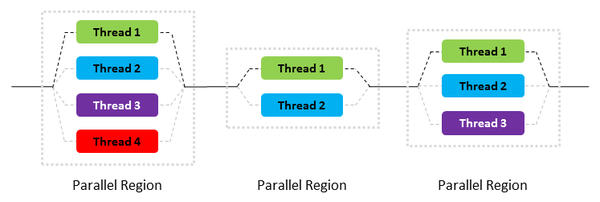
\includegraphics[scale=0.5]{img/pic1.jpg}
   \caption{Mô hình Fork-Join}
   \label{fig:pic_fork_join}
\end{figure}

\begin{description}
\item [Fork] Có nghĩa là luồng chủ sau đó sẽ tạo ra một tập các luồng song song. Và sau đó đoạn mà trong vùng song song được thực thi song song bởi tập luồng song song vừa tạo ra 
\item [Join] Khi mà tập luồng song song đã hoàn thành đoạn mã trong vùng song song chúng sẽ được đồng bộ và kết thúc rồi sau đó công việc lại được thực hiện bởi luồng chủ.
\end{description}


\section{Các khuôn dạng chỉ thị trong OpenMP}
\subsection{Khuôn dạng chỉ thị trong OpenMP}
Chỉ thị trong OpenMP dược cho dưới dạng sau:
\begin{verbatim}
	#pragma omp directive-name [clause...] newline
\end{verbatim}

\begin{itemize}
\item \textsf{\#pragma omp}: Yêu cầu bắt buộc với mọi chỉ thị OpenMP C/C++
\item \textsf{directive-name}: Là tên của chỉ thị phải xuất hiện sau \textsf{\#pragma omp} và đứng trước bất kì mệnh đề nào
\item \textsf{[clause...]}: Là các mệnh đề, không bắt buộc có trong chỉ thị
\item \textsf{newline} Yêu cầu bát buộc với mỗi chỉ thị.
\end{itemize}
Ví dụ:
\begin{minted}{C}
#pragma omp parallel default(shared) private(i)
\end{minted}


\subsection{Phạm vi của chỉ thị}
\begin{description}
\item [Phạm vi tĩnh] Đó là nhngx đoạn mã nguyên bản trong phạm vi từ đầu đến cuối cấu trúc cho sau mỗi chỉ thị. Phạm vi tĩnh của chỉ thị không mở rộng dến các thủ tục và các tệp chứa mã.
\item [Chỉ thị đơn độc] Chỉ thị đơn đọc là chỉ thị xuất hiện độc lập với chỉ thị khác. Nó tồn tại ở ngoài phạm vi tĩnh của chỉ thị khác. Chỉ thị đơn độc mở rộng với các thủ tục và tệp mã nguồn.
\item[Phạm vi động] Phạm vi động của chỉ thị bao gồm phạm vi tĩnh của chỉ thị và phạm vi của các chỉ thị mồ côi.
\end{description}
\begin{figure}[htp]
\centering
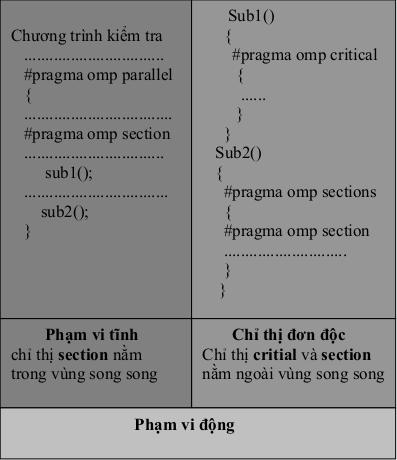
\includegraphics[scale=0.5]{img/pic2.png}
\caption{Phạm vị của chỉ thị}
\label{pic_pv_chithi}
\end{figure}

\subsection{Cấu trúc một vùng song song}
Một vùng song song là một khối mã được thực thi bởi nhiều luồng. Trong C/C++ một vùng song song có định dạng như sau:

\begin{minted}[frame=single, linenos=true, tabsize=4]{C}
#pragma omp parallel [clause] newline
	if (scalar_expression)
	private (list)
	shared(list)
	default(shared | none)
	firstprivate(list)
	reduction(operator:list)
	copyin(list)
	structed_block
\end{minted}

Ví dụ:
\begin{minted}[frame=single, linenos=true, tabsize=4]{C}
#prabma omp parallel
	printf("Hello");
	\end{minted}
	
	
\begin{figure}[htp]
\centering
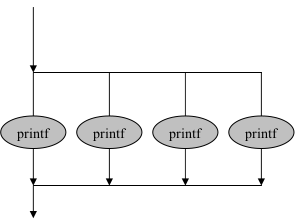
\includegraphics[scale=0.6]{img/pic3.png}
\caption{Sự thực thi đồng thời của các luồng trong cấu trúc vùng song song}
\end{figure}

Khi mà một luồng gặp chỉ thị \textsf{parallel} thì nó sẽ tạo ra một tập các luồng
và luồng ban đầu sẽ là luồng chủ của tập các luồng đó. Luồng chủ ở đây cũng là một
thành viên trong tập các luồng đó và là luồng số 0.

Để bắt đầu thực hiện một vùng song song thì đoạn mã nguồn trong vùng song
song được sao ra những bản giống nhau đưa cho mỗi luồng thực hiện một cách song
song. Đợi cho đến khi tất cả các luồng đều thực hiện song công việc của mình thì
luồng chủ sẽ thực hiện công việc tuần tự còn lại ngoài vùng song song đó. Vậy câu hỏi
đặt ra ở đây là có bao nhiêu luồng để thực hiện đoạn mã song song trong vùng song song. 
Để biết được điều này người ta dùng hàm thư viện \textsf{OMP\_NUM\_THREAD()}, và để biết được số thứ tự của mỗi luồng ta dùng hàm \textsf{OMP\_GET\_THREAD\_NUM()}... Lưu ý số thứ tự của các luồng nằm trong khoảng từ 0 đến số thứ tự của luồng chủ trừ đi 1. Cũng từ khái niệm vùng song song xuất hiện khái niệm vùng song song lồng và khái niệm luồng động
\begin{description}
\item [Vùng song song lồng (Nested Parallel Region)]: Có nghĩa là trong một vùng
song song con xuất hiên các vùng song song nhỏ khác.
\item [Luồng động (Dynamic Thread)] Theo mặc định thì khi một chương trình được
chia ra thành nhiều vùng song song thì các vùng song song đó sẽ được thực hiện bởi
các luồng với số lượng bằng nhau. Điều này có thể thay đổi bằng cách cho phép hệ
thống gán động số lượng các luồng thực hiện cho mỗi vùng song song . Chúng ta có
hai cách thức để gán động các luồng thứ nhất là dùng hàm thư viện
\textsf{omp\_set\_dynamic()} và thứ hai là dùng biến môi trường \textsf{OMP\_DYNAMIC}.
\end{description}
\begin{figure}[htp]
	\centering
	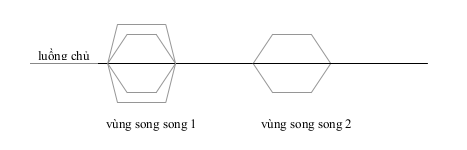
\includegraphics[scale=0.6]{img/pic4.png}
	\caption{Cấu trúc phân chia luồng động}
	\end{figure}

\subsection{Cấu trúc chia sẻ công việc}
Cấu trúc chia sẻ công việc dùng để chia việc thực hiện công việc trong vùng
song song cho các luồng trong tập các luồng thực hiện công việc cho bởi vùng song
song. Cấu trúc chia sẻ công việc phải được bao bọc bởi một vùng song song để có thể
thực hiện song song và cấu trúc này có thể được thực hiện bởi tất cả các luồng trong
tập các luồng hoặc chỉ một số luồng trong tập các luồng thực thi vùng song song. Có
ba loại cấu trúc chia sẻ công việc đó là cấu trúc \textsf{DO/for}, cấu trúc {SECTIONS} và cấu trúc {SINGLE}

\subsubsection{Chỉ thị DO/for}
Chỉ thị \textsf{DO/for} chỉ ra rằng các công việc lặp đi lặp lại (interations) cho bởi
vòng lặp phải được các luồng thực hiện một cách song song. Chỉ thị for trong C/C++
được cho dưới dạng sau:
\begin{minted}[frame=single, tabsize=4]{C}
#pragma omp for [clause...] newline
	schedule ( type [,chunk\_size] )
	ordered
	private ( list )
	firstprivate ( list )
	lastprivate ( list )
	shared ( list )
	reduction ( operator : list )
	nowait
for_loop
\end{minted}

\paragraph{Mệnh đề SCHEDULE}
Mệnh đề này chỉ ra rằng các công việc lặp đi lặp lại (interations) của vòng lặp
được phân chia cho các luồng thực hiện như thế nào. Có ba kiểu phân chia.
\begin{description}
	\item[STATIC] Đối với kiểu phân chia này thi các công việc của vòng lặp đi lặp lại của vòng lặp được phân chia dựa theo giá trị của biến \emph{chunk\_size} thành các \emph{chunk} công việc liên tiếp (mỗi \emph{chunk} công việc ở đây bao gồm \emph{chunk\_size} các công việc lặp đi lặp lại) và gán tĩnh \emph{chunk} công việc này cho các luồng thực hiện theo kiểu quay vòng dựa trên thứ tự của số hiệu mỗi luồng. Nếu biến chunk không được chỉ định thì các công việc này sẽ được phân chia lần lượt cho các luồng.
	Ví dụ:
	\begin{minted}[frame=single, tabsize=4]{C}
	#pragma omp parallel for schedule(static, 2)
		for (int i=1; i<8; i++)
			a[i] = i;
	\end{minted}
	\begin{figure}[htp]
		\centering
		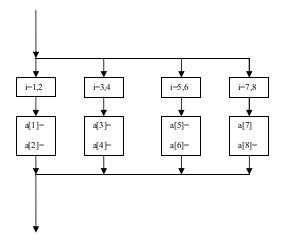
\includegraphics[scale=1.0]{img/pic5.png}
		\caption{Mô tả hoạt động với schedule static}
		\end{figure}
	\item[DYNAMIC]
	Đối với việc phân chia động thì các công việc lặp đi lặp lại của vòng lặp được
	phân chia thành một chuỗi các \emph{chunk}. Mỗi \emph{chunk} ở đây là một tập \emph{chunk\_size} công việc. Các \emph{chunk} này sẽ được gán động cho mỗi luồng. Các luồng sau khi kết thúc một \emph{chunk} công việc sẽ đợi để nhận \emph{chunk} công việc cho đến khi không còn \emph{chunk} công việc nào được gán. Lưu ý rằng \emph{chunk} công việc cuối cùng có thể có số lượng công việc nhỏ hơn \emph{chunk\_size}. Nếu biến \emph{chunk\_size} không được chỉ ra thì giá trị mặc định của nó là 1.
	Ví dụ:
		\begin{minted}[frame=single, tabsize=4]{C}
		#pragma omp parallel for schedule(dynamic, 2)
		for (int i=1; i<8; i++)
		a[i] = i;
		\end{minted}
			\begin{figure}[htp]
				\centering
				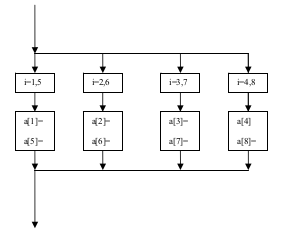
\includegraphics[scale=1.0]{img/pic6.png}
				\caption{Mô tả hoạt động với schedule dynamic}
			\end{figure}
	\item[GUIDED]
	Kiểu phân chia này tương tự như kiểu phân chia động chỉ khác ở chỗ cỡ của mỗi \emph{chunk} công việc không phải là hằng số mà nó giảm đi theo hàm mũ qua mỗi lần một luồng thực hiện song một \emph{chunk} công việc và bắt đầu thực hiện một \emph{chunk} công việc mới. Khi mà một luồng kết thúc một \emph{chunk} công việc nó sẽ được gán động sang một \emph{chunk} khác. Với \emph{chunk\_size} là 1 thì cỡ của \emph{chunk} công việc được tính băng phép chia nguyên số lượng công việc cho số các luồng thực hiện và cỡ này sẽ giảm dần cho đến 1. Còn nếu \emph{chunk\_size} có giá trị k thì cỡ của \emph{chunk} công việc sẽ giảm dần cho đến k. Chú ý cỡ của \emph{chunk} cuối cùng có thể nhỏ hơn k. Khi mà giá trị của \emph{chunk\_size} không được khởi tạo thì giá trị mặc định của nó là 1.
	Ví dụ:
	\begin{minted}[frame=single, tabsize=4]{C}
	#pragma omp parallel for schedule(guided, 2)
		for (int i=1; i<37; i++)
			a[i] = i;
	\end{minted}
	\begin{figure}[htp]
		\centering
		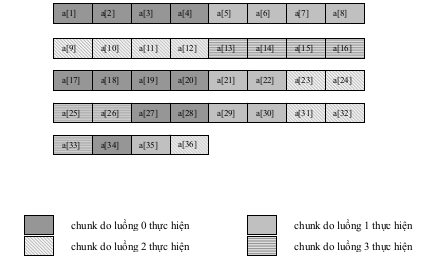
\includegraphics[scale=1.0]{img/pic7.png}
		\caption{Mô tả hoạt động với schedule guided với 37 bước lặp}
	\end{figure}
	\item[RUNTIME]
	Khi mà bắt gặp \emph{schedule (runtime)} thì công việc lập lịch bị hoãn lại cho tới
	khi \emph{runtime}. Kiểu phân chia và cỡ của các \emph{chunk} có thể được thiết lập tại thời điểm \emph{runtime} bằng một biến môi trường có tên gọi \textsf{OMP\_SCHEDULE}. Nếu biến môi trường này không được thiết lập thì việc lập lịch chia sẻ công việc sẽ được thực hiện mặc định. Khi mà \emph{schedule (runtime)} được đưa ra thì \emph{chunk\_size} không được khởi tạo
	\end{description}

\paragraph{Mệnh đề ORDERED}
	Mệnh đề này chỉ được xuất hiện khi có chỉ thị ORDERED được bao bọc bởi chỉ thị \textsf{DO/for}
\paragraph{Mệnh đề NOWAIT}
Với mệnh đề này thì tất cả các luồng không cần đồng bộ tại điểm cuối cùng
của vòng lặp song song. Các luồng sẽ xử lý trực tiếp đoạn mã lệnh cho tiếp sau vòng
lặp. Các mệnh đề còn lại sẽ được thảo luận ở phần sau.

\subsubsection{Chỉ thị SECTIONS}
Chỉ thị này dùng để chỉ ra các phần mã trong vùng song song chia cho các
luồng thực hiện. Trong phạm vi của chỉ thị \textsf{SECTIONS} có các chỉ thị textsf{SECTION}. Mỗi
một textsf{SECTION} sẽ được thực hiện bởi một luồng trong tập các luồng và các textsf{SECTION}
khác nhau sẽ được thực hiện bởi các luồng khác nhau. Trong C/C++ chi thị
textsf{SECTIONS} được cho dưới dạng sau

\begin{minted}[frame=single, tabsize=4]{C}
#pragma omp sections [clause...]
	private(list)
	firstprivate(list)
	lastprivate(list)
	reduction(operator:list)
	nowait
{
#pragma omp section
	structured_block
#pragma omp section
	structured_block
}
\end{minted}

\subsubsection{Chỉ thị SINGLE}
Mệnh đề SINGLE chỉ ra rằng đoạn mã bao quanh chỉ thị được thực hiện bởi một luồng trong tập các luồng.Trong C/C++ chỉ thị \textsf[SINGLE] được cho dưới dạng như sau:
\begin{minted}[frame=single, tabsize=4]{C}
#pragma omp single [clause...]
private(list)
firstprivate(list)
nowait
\end{minted}
 Các luồng khác mà không thực thi đoạn mã trong chỉ thị \textsf{SINGLE} sẽ phải đợi đến khi luồng thực thi đoạn mã trong chỉ thị kết thúc mới được thực hiện các công việc ngoài chỉ thị \textsf{SINGLE} nếu mệnh đề \textsf{NOWAIT} được đưa ra. Lưu ý trong chỉ thị \textsf{SINGLE} chỉ có hai mệnh đề là private và firstprivate.
 
 \subsection{Cấu trúc đồng bộ}
\subsubsection{Chỉ thị MASTER}
Trong chỉ thị \textsf{MASTER}, đoạn mã bao quanh chỉ thị chỉ được thực hiện bởi luồng chủ trong tập các luồng. Trong chỉ thị loại này không có bất cứ mệnh đề nào và các luồng khác không cần chờ đến khi luồng chủ thực hiện xong công việc cho bởi chỉ thị master mới được thực hiện công việc của mình. Trong C/C++ chỉ thị được cho dưới dạng:
\begin{minted}[frame=single, tabsize=4]{C}
#pragma omp master
	structure_block
	\end{minted}
	
	\subsubsection{Chỉ thị CRITICAL}
	Với chỉ thị \textsf{CRITICAL} thì vùng mã được cho bởi chỉ thị tại một điểm chỉ được thực hiện bởi một luồng. Ta lưu ý rằng nếu có một luồng đăng thực hiện công  việc cho bởi chỉ thị mà có một luồng khác cố gắng đòi thực hiện cong việc đó thì nó sẽ bị khóa cho đến khi luồng kia thực hiện xong công việc đó. Một chú ý nữa là có thể tồn tại nhiều chỉ thị \textsf{CRITIAL} với các tên khác nhau trong một vùng song song. Tên của chỉ thị được nhận dạng một cách toàn cục, tất cả các vùn g \textsf{CRITIA}L với tên giống nhau được coi như là cùng một vùng. Tất cả vùng \textsf{CRITIAL} không có tên cũng được coi như cùng một vùng. Trong C/C++ chỉ thị này được cho dưới dạng: 
	\begin{minted}[frame=single, tabsize=4]{C}
	#pragma omp critical [name] 
	structure_block
	\end{minted}
	
	\subsubsection{Chỉ thị ATOMIC}
	Trong chỉ thị \textsf{ATOMIC}, các địa chỉ vùng nhớ dược cập nhật một cách nguyên tố hơn là việc dùng nhiều luồng cố gắng ghi đè lên nó.Trong C/C++ chỉ thị này được cho dưới dạng:
	\begin{minted}[frame=single, tabsize=4]{C}
	#pragma omp atomic
	statement_expression
	\end{minted}

\subsubsection{Chỉ thị BARRIER}
Chỉ thị \textsf{BARRIER} dùng để đồng bộ tất cả các luồng trong tập các luồng. Khi bắt gặp chỉ thị \textsf{BARRIER} thì ubmỗi một luồng sẽ chờ đợi tại thời điểm đấy cho đến khi tất cả các luồng còn lại đều bắt gặp chỉ thị \textsf{BARRIER}. Và sau đó tất cả các luồng sẽ thực hiện đoạn mã hco bởi chỉ thị \textsf{BARRIER}. Trong C/C++ chỉ thị \textsf{BARRIER} được cho dưới dạng sau: 
\begin{minted}[frame=single, tabsize=4]{C}
#pragma omp barrier 
structure_block
\end{minted}

\subsubsection{Chỉ thị ORDERED}
Chỉ thị \textsf{ORDERED} được đưa ra để đảm bảo rằng các công việc của vòng lặp phải được thực hiện đúng theo thứ tự khi chúng được thực thi tuần tự. Một chỉ thị \textsf{ORDERED} chỉ có thể xuất hiện trong phạm vi động của chỉ thị for hoặc parallel for trong C/C++. Và tại bất cứ thời điểm nào thì chỉ có một luồng thực hiện đoạn mã cho bởi chỉ thị \textsf{ORDERED}. Nếu một vòng lặp có chỉ thị này thì nhất định nó phải chứa mệnh đề \textsf{ORDERED}. Trong C/C++ chỉ thị được cho dưới dạng sau: 
\begin{minted}[frame=single, tabsize=4]{C}
#pragma omp ordered
structure_block
\end{minted}

\subsubsection{Chỉ thị THREADPRIVATE}
Chỉ thị này được dùng để tạo ra các biến có phạm vi toàn cục trong một file để
các biến đó có thể được sử dụng ở nhiều vùng song song trong một file chương trình
và chúng được bảo vệ bởi mỗi luồng. Trong C/C++ chỉ thị được cho dưới dạng sau
\begin{minted}[frame=single, tabsize=4]{C}
#pragma omp threadprivate(list)
\end{minted}
Chú ý rằng trong chương trình chỉ thị này phải xuất hiện sau dòng lệnh khai
báo các biến toàn cục. Mỗi một luồng sau đó sẽ tạo ra một bản sao của biến đó để mà
việc thay đổi biến thuộc luồng nay không ảnh hưởng tới biến đó thuộc luồng khác
Ví dụ:
\begin{minted}[frame=single, tabsize=4]{C}
#include <omp.h>
int alpha[10], beta[10], i;
#pragma omp threadprivate(alpha)
main ()
{
/* mở một luồng động */
	omp_set_dynamic(0);
/* vùng song song một */
#pragma omp parallel private(i,beta)
	for (i=0; i < 10; i++)
		alpha[i] = beta[i] = i;
/* vùng song song hai */
#pragma omp parallel
	printf("alpha[3]= %d and beta[3]= %d\n",alpha[3],beta[3]);
\end{minted}

\subsection{Các mênh đề trong OpenMP}
Vì OpenMP lập trình trên máy tính chia sẻ bộ nhớ chung nên việc hiểu và sử
dụng được phạm vi của các biến trong chương trình là rất quan trọng. Phạm vi của các
biến ở đây bao gồm hai phạm vi toàn cục và phạm vi bảo vệ. Các biến toàn cục bao
gồm các biến tĩnh và biến file toàn cục còn các biến bảo vệ bao gồm biến chỉ số trong
vòng lặp, biến trong thủ tục được gọi từ vùng song song. Các mệnh đề về phạm vi dữ
liệu bao gồm các mệnh đề sau:
\begin{itemize}
	\item PRIVATE
	\item FIRSTPRIVATE
	\item LASTPRIVATE
	\item SHARED
	\item DEFAULT
	\item REDUCTION
	\item COPYIN
	\end{itemize}
Các mệnh đề về phạm vi dữ liệu này được sử dụng với một vài chỉ thị
(PARALLEL, FOR, SECTIONS ) để điều khiển phạm vi các biến trong các
chỉ thị đó. Sau đây ta sẽ đi vào chi tiết từng mệnh đề.

\subsubsection{Mệnh đề PRIVATE}
Mệnh đề này dùng để khai báo các biến trong danh sách các biến dùng riêng
cho mỗi luồng . Mỗi luồng sẽ sử dụng một bản sao của biến \textsf{PRIVATE} và có quền sử dụng độc lập đối với biến đó . Trong C/C++ nó được khai báo như sau:
\textsf{private (list)}
\subsubsection{Mệnh đề FIRSTPRIVATE}
Mệnh đề này cũng dùng để khai báo một danh sách các biến dùng riêng cho
mỗi luồng giống như ở mệnh đề \textsf{PRIVATE}. Nhưng nó khác mệnh đề \textsf{PRIVATE} ở chỗ
các bản sao của mỗi biến dùng cho mỗi luồng được khởi tạo một giá trị ban đầu trước
vùng song song hoặc cấu trúc chia sẻ công việc. Trong C/C++ mệnh đê trên được khai
báo như sau:
\textsf{firstprivate (list)}
\subsubsection{Mệnh đề LASTPRIVATE}
Mệnh đề này cũng được dùng để khai báo một danh sách các biến dùng riêng
cho mỗi luồng như ở mệnh đề \textsf{PRIVATE}. Nhưng nó khác mệnh đề \textsf{PRIVATE} ở chỗ
giá trị của biến chính là giá trị của biến dùng riêng của luồng thực hiện công việc cuối
cùng của vòng lặp hoặc section cuối cùng trong chỉ thị sections. Trong C/C++ mệnh
đề trên được khai báo như sau: \textsf{lastprivate (list)}

\subsubsection{Mệnh đề SHARED}
Mệnh đề này dùng để khai báo các biến trong danh sách các biến được chia sẻ
cho tất cả các luồng trong tập các luồng. Các biến chia sẻ chỉ có một vị trí trong bộ
nhớ và các luồng sẽ đọc và ghi trên cùng một vị trí đấy. Việc các luồng cùng đọc và
ghi lên cùng một vị trí trên bộ nhớ rất có thể dẫn đến sai xót trong chương trình nên
người lập trình phải chịu trách nhiệm phân bố công việc cho mỗi luồng một cách hợp
lý (ví dụ như thông qua chỉ thị \textsf{CRITIAL}). Trong C/C++ mệnh đề trên được khai báo như sau
\textsf{shared (list)}

\subsubsection{Mệnh đề DEFAULT}
Mệnh đề này cho phép người lập trình đưa ra phạm vi \textsf{PRIVATE, SHARED},
hoặc \textsf{NODE} cho tất cả các biến thuộc vàophạm vi của bất kỳ vùng song song nào. Và chỉ có chỉ thị \textsf{DEFAULT} mới được đưa ra trong cấu trúc vùng song song. Trong
C/C++ chỉ thị này được khai báo như sau:
\textsf{default (shared |none)}
\subsubsection{Mệnh đề REDUCTION}
Mệnh đề này được dùng để thu gọn các biến có ở trong danh sách các biến.
Một bản sao của mỗi biến cho bởi danh sách các biến sẽ được tạo ra cho mỗi luồng.
Tại thởi điểm cuối cùng của việc thu gọn thì các phép toán thu gọn sẽ được áp dụng
nên các bản sao dùng riêng của mỗi luồng. Và kết quả cuối cùng được lưu vào biến
chia sẻ toàn cục. Trong C/C++ mệnh đề trên được khai báo như sau:
\textsf{reduction (operator: list)}.
Chý ý các biến trong danh sách phải là các biến vô hướng. Chúng không thể là
các biến kiểu mảng hoặc kiểu có cấu trúc và chúng phải được khai báo là biến chia sẻ.

\subsubsection{Mệnh đề COPYIN}
Mệnh đề này dùng để gán giá trị của biến \textsf{THREADPRIVATE} cho từng luồng
trong tập các luồng thực thi một vùng song song. Có nghĩa là giá trị của biến
\textsf{THREADPRIVATE} được khai báo trong mệnh đề \textsf{COPYIN} của luồng chủ sẽ được
dùng làm nguồn. Khi gặp một vùng song song thì biến nguồn này sẽ được sao cho các
luồng thực thi vùng song song đó. Lưu ý rằng các biến khai báo trong mệnh đề
\textsf{COPYIN} là các biến \textsf{THREADPRIVATE}. Trong C/C++ mệnh đề trên được khai báo
như nhau:
\textsf{copyin (list)}

\section{Thư viện runtime}
OpenMP cung cấp một thư viện với rất nhiều các hàm chức năng bao gồm các
truy vấn liên quan đến số lượng và chỉ số các luồng, thiết lập số lượng các luồng sử
dụng, semaphores, và các hàm thiết lập môi trường thực thi. Trong C/C++ để có thể sử
dụng các hàm trên thì phải đính vào file thư viện \emph{omp.h}. Sau đây ta đi vào chi tiết các từng hàm thư viện một.

\begin{tabular}{|p{7cm}|p{5cm}|}
	\hline  void omp\_set\_num\_threads(int num\_threads)&  Thiết lập số các luồng thực hiện vùng song song. \\
	\hline int omp\_get\_num\_thread() & Số luồng thực hiện vùng song song \\ 
	\hline int omp\_get\_max\_threads() & Trả về giá trị lớn nhất trong các giá trị trả về của hàm omp\_get\_umum\_thread() \\
	\hline  int omp\_get\_thread\_num()& Trả về chỉ số của luồng đang thực hiện  \\ 
	\hline  int omp\_get\_num\_procs()& Tả về số lượng các bộ xử lý đang thực thi chương trình tại thời điểm được gọi  \\ 
	\hline int omp\_in\_parallel & Kiểm tra xem vùng mã chứa dnos được thực hiện song song hay tuần tự  \\ 
	\hline void omp\_set\_dynamic(int dynic\_thead) & Diều khiển sự cho phép hoặc không cho phép sự điều chỉnh động của các luồng thực thi trong vùng song song \\ 
	\hline  int omp\_get\_dynamic()&  Kiểm tra xem có sự điều chỉnh động hay không \\ 
	\hline void omp\_set\_nested(int nested) & Cho pép hay không cho pép việc song song lồng \\ 
	\hline int omp\_get\_netsted() &  Kiểm tra sự cho phép hay không cho phép song song lồng \\ 
	\hline
	
\end{tabular} 

\section{Các biến môi trường}
Các biến môi trường dùng để điều khiển sự thực hiện các đoạn mã song song. Bao gồm các biến môi trường sau:
\begin{description}
	\item [OMP\_SCHEDULE] Biến này chỉ được sử dụng trong chỉ thị có kiểu lập lịch RUNTIME như chỉ thị for và parallel for. Giá trị của biến này để xác định xem các công việc trong vòng lặp được lập lịch trên các BXL như thế nào
	\item [OMP\_NUM\_THREADS] Thiết lập số lượng lớn nhất các luồng được sử dụng
	\item [OMP\_DYNAMIC] Biến này cho phép hay không sự điều chỉnh động cho các luồng thực thi các vùng song song. Nó nhận hai giá trị TRUE hoặc FALSE.
	\item [OMP\_NESTED]Cho phép hay không việc song song lồng xảy ra.
	\end{description}


\chapter{Giải thuật Collaborative Fittering cho Recommender System}

\section{Tổng quan về Recommender System - Hệ tư vấn}
\subsection{Giới thiệu về hệ tư vấn}
Trong cuộc sống hàng ngày, trong rất nhiều trường hợp, người ta đưa ra các lựa chọn
dựa trên những ý kiến hay lời khuyên của mọi người xung quanh, có thể qua lời nói,
các bản đánh giá sản phẩm, khảo sát thị trường, thư giới thiệu ...v..v. Nhưng trong kỉ
nguyên thông tin, hàng triệu thông tin được đưa lên internet mỗi ngày, điều này dẫn
tới yêu cầu phải có các phương pháp tự động thu thập thông tin và đưa ra lời khuyên
để hỗ trợ cho các phương pháp truyến thống trên . Hệ tư vấn \emph{recommender system} là một giải pháp như vậy. Hệ thống này đưa ra gợi ý dựa trên những gì người dùng đã
làm trong quá khứ, hoặc dựa trên tổng hợp ý kiến của những người dùng khác. Hệ tư
vấn đã trở thành một ứng dụng quan trọng và thu hút được sự quan tâm lớn của các
nhà nghiên cứu cũng như các doanh nghiệp.
Một vài hệ tư vấn nổi tiếng:
\begin{description}
	\item[Phim/TV/Âm nhạc] MovieLens, EachMovie, Firefly, Fycastingycasting, Ringo...
	\item[Tin tức/ báo chí] Tapetry, GroupLens, Lotus Notes, Anatagonomy, ...
	\item [Sách / Tài liệu] Amazone.com, oFoxtrot, InfoFinder, ...
	\item [Web] Phoaks, Gab, Fab, IfWeb, ....
	\item [Nhà hàng] Adaptive Place Advisor, Polylens, Pocket restaurent finder, ...
	\item [Du lịch] Dietorecs, LifestyleFinder, ...
	\end{description}

\subsection{Bài toán tư vấn}
Bài toán tư vấn được coi là bài toán ước lượng trước hạng (rating) của các sản phẩm (phim, cd, nhà hàng, ...) chưa được người dùng xem xét. Việc ước lượng này thường dựa trên những đánh giá đã có của chính người dùng đó hoặc những người dùng khác. Những sản phẩm có hạng cao nhất sẽ được dùng để tư vấn.
\subsection{Phân loại hệ tư vấn}
Có rất nhiều cách để dự đoán, ước lượng hạng/điểm cho các sản phẩm như sử dụng học máy, lý thuyết xấp xỉ, các thuật toán dựa trên kinh nghiệm. Các hệ thống tư vấn thường được phân thành 3 loại dựa trên cách nó dùng để ước lượng sản phẩm:
\begin{itemize}
	\item Content-based (dựa trên nội dung): Người dùng được gợi ý những sản phẩm tương tự các sản phẩm từng được họ đánh giá cao.
	\item Collaborative (dựa trên cộng tác): Người dùng được gợi ý những sản phẩm mà những người cùng sở thích với họ đánh giá cao
	\item Hybrid (lai ghép): Kết hợp cả hai phương pháp
\end{itemize}

\section{Giải thuật Collaborativeollaborative filering}
\emph{Collaborative filtering} (CF) là một giải thuật cho hệ tư vấn phố biến.
Ý tưởng cơ bản của các hệ thống này là dựa vào các đánh giá của những người dùng quá khứ lên các sản phẩm, dịch vụ để dự đoán sự đánh giá của họ lên các sản phẩm, dịch vụ mà họ chưa đánh.
Bài toán lọc cộng tác (hay đánh giá độ tương quan) dựa trên hành vi quá khứ của người dùng (trong việc đánh giá sản phẩm) để đưa ra dự đoán.
Đầu vào của bài toán là ma trận thể hiện những hành vi quá khứ, gọi là ma trận Người dùng- Sản phẩm (m trận User x Item). Hàng là người dùng, cột là sản phẩm, giá trị mỗi ô là đánh giá của người dùng lên sản phẩm đó.

/emph{Tùy theo hệ thống mà đánh giá của người dùng được quy ước những giá trị nào. Trong ví dụ này, các đánh giá có giá trị từ 1-5}

\begin{tabular}{|c|c|c|c|}
	\hline  & Sản phẩm 1 & Sản phẩm 2 & Sản phẩm 3 \\ 
	\hline Người dùng 1 & 1 &  0& 5 \\ 
	\hline Người dùng 2 & 4 & 2 & 2 \\ 
	\hline  Người dùng 3 &  0& 0 & 0  \\ 
	\hline 
\end{tabular} 

Ở ma trận này, đánh giá của người dùng 1 đối sản phẩm 1 là 1, sản phẩm 3 là 5,
sản phẩm 2 chưa được đánh giá.

Đầu ra của bài toán là: đánh giá của người dùng lên những sản phẩm mà họ
chưa đánh giá. Hệ thống khuyến nghị dựa trên các đánh giá này mà xếp hạng các sản
phẩm và gợi ý cho người dùng.

Trong ví dụ này, hệ thống khuyến nghị phải đưa ra dự toán, người dùng 1 đánh
giá sản phẩm 2 là bao nhiêu. Người dùng 3 đánh giá sản phẩm 1, 2, 3 là bao nhiêu.


Hệ thống khuyến nghị lọc cộng tác dự đoán độ phù hợp \emph{r(u,i)} của một sản
phẩm \emph{i} với người dùng \emph{u} dựa trên độ phù hợp \emph{r(ui,i)} giữa người dùng \emph{ui} và \emph{i}, trong đó \emph{ui} là người có cùng sở thích với \emph{u}. Ví dụ, để gợi ý một bộ phim cho người dùng\emph{u}, đầu
tiên hệ thống cộng tác tìm những người dùng khác có cùng sở thích phim ảnh với {u}.
Sau đó, những bộ phim được họ đánh giá cao sẽ được dùng để tư vấn cho u. Có nhiều
hệ thống cộng tác đã được phát triển như: Youtube (video), Amazon.com (sách)... Các
hệ thống này có thể chia thành hai loại: dựa trên kinh nghiệm (heuristic-based hay
memory-based) và dựa trên mô hình (model-based).


\subsection{Ưu điểm}
\begin{itemize}
	\item \emph{Không giới hạn về loại đối tượng dùng để khuyến nghị}: Phương pháp CF hoàn toàn dựa vào đánh giá của người dùng để đưa ra các nhận định về sở thích của người dùng. Chính vì thế các tính cất của đối tượng được khuyến nghị không ảnh hưởng đến quá trình khuyến nghị. Ưu điểm này giúp phương pháp lọc cộng tác được áp dụng đa dạng trên nhiều hệ thống khác nhau từ trang thông tin đến âm nhạ, hình ảnh...
	\item \emph{Khuyến nghị đa dạng}: Khắc phục được giới hạn của phương pháp tiếp cận dựa trên nội dung, , phương pháp Lọc cộng tác có thể đưa ra các đối tượng sản phẩm khuyến nghị hoàn toàn khác so với các sản phẩm mà
	người dùng U đã thích trong quá khứ.
	\end{itemize}
\subsection{Nhược điểm}
\begin{itemize}
	\item \emph{Cold Start}: Cần một lượng người dùng nhất định trong hệ thống để có thể tìm kiếm sự tương đồng giữa các người dùng.
	\item \emph{Sparsity} Số lượng user/rating quá thưa, khó có thể tìm kiếm được những người dùng cùng bình chọn item giống nhau
	\item \emph{First rater} Xử lý với user mới, hoặc item mới.
	\item \emph{Popularity bias} Thường kuyến nghị những item phổ biến.
	\end{itemize}

	
\section{Cài đặt}	
Cài đặt giải thuật CF gồm có các bước cơ bản sau:
\begin{itemize}
	\item Chuẩn hóa ma trận rating(user*item)
	\item Tính similary giữa các user/item
	\item Chọn ra số lượng lân cận và dự đoán
	\end{itemize}
	
	\subsection{Vấn đề chuẩn hóa}
	\begin{description}
	\item [Phương pháp Mean-Centering]: Ý tưởng chính của phương
	pháp này là so sánh một Đánh giá của người dùng là âm
	hay dương (tốt hay xấu) so với Đánh giá trung bình.
	$$H (r_{ui}) = r_{ui} - r_{ui}$$
	Nhược điểm của phương pháp này là khi hai người dùng A
	và B có cùng giá trị trung bình của các đánh giá, thì sự
	phản ảnh của 2 người dùng này là giống nhau mặc dù trên
	thược tế người dùng A có thể có các đánh giá 2,3,4 trong
	khi người dùng B lại có cả 3 đánh giá đều mang giá trị là 3.
	\item [Phương pháp Z-Score]:
	Phương pháp này khắc phục được nhược điểm của phương
	pháp Mean-Centering. Phương pháp này phân hóa các
	đánh giá là tốt hay xấu dựa trên độ lệch chuẩn của các
	đánh giá.
	$$H (r_{ui}) = (r_{ui} - r_i) / o_i$$
	\end{description}
	
	\subsection{Phương pháp tính độ tương tự}
	Có nhiều cách để tính độ tương đồng về sở thích giữa hai người dùng nhưng trong hầu hết các phương pháp, độ tương đồng chỉ được tính dựa trên các sản phẩm được cả hai người cùng đánh giá. Hai phương pháp phổ biến nhất là dựa trên độ tương quan và dựa trên cosin.
	
	Với phương pháp dựa trên cosin, hai người dùng được biểu diễn bởi 2 vector m chiều. Độ tương đồng giữa 2 vector được tính bởi công thức:
	\begin{figure}[htp]
		\centering
		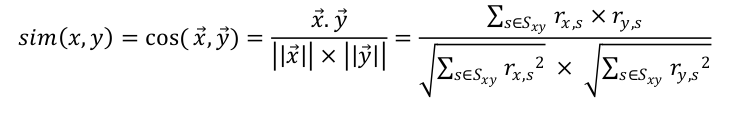
\includegraphics[scale=0.4]{img/pic8.png}
	\end{figure}
	
	\subsection{Chọn số lượng lân cận}
	Việc lựa chọn số lượng lân cận là rất quan trọng vì nó ảnh hưởng trực tiếp đến chất
	lượng của khuyến nghị. Nếu chọn số lượng lân cận lớn rõ ràng chất
	lượng của khuyến nghị sẽ được nâng lên. Tuy nhiên, đi theo đó là các chi
	phí về bộ nhớ, thời gian tính toán cũng phải tăng theo. Ngược lại, nếu
	lựa chọn số lân cận quá thấp thì sẽ ảnh hưởng đến chất lượn của khuyến
	nghị. Có một vài phương pháp nhằm giải quyết việc lựa chọn như sau:
	\begin{itemize}
		\item Chọn top-N: chọn N lân cận có độ tương đồng cao nhất.
		\item Chọn theo ngưỡng: Định ra một ngưỡng cho độ tương đồng, các lân cận nào có độ tương dồng vượt qua ngưỡng thì được lưu trữ lại và tính toán.
		\item Tính âm.
		\end{itemize}
	
	\subsection{Kết hợp global baseline estimate}
		$$b_{ui} = u + b_u + b_i$$
		Trong đó:
		\begin{itemize}
			\item $b_ui$: Giá trị đánh giá ước lượng.
			\item $u$: Giá trị trung bình đánh giá của người dùng trên toàn bộ các sản phẩm.
			\item $b_u$ Là giá trị phương sai của các đánh giá của người dùng u.
			\item $b_i$ Là giá trị phương sai của các đánh giá trên sản phẩm i.
		\end{itemize}
		
		Kết quả đánh giá cuối cùng khi kết hợp cả hai phương pháp được tính theo công thức:
		\begin{figure}
			\centering
			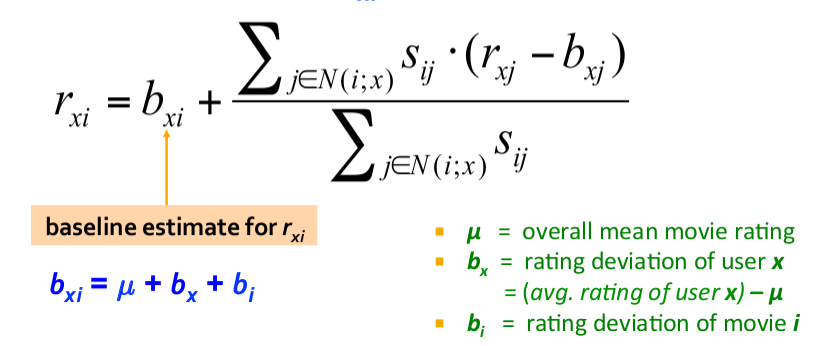
\includegraphics[scale=0.5]{img/pic9.png}
			\caption{Công thức đánh giá dựa trên cả hai phương pháp}
		\end{figure}
		
	
	\section{Kết quả thực nghiệm}
	\subsection{Đánh giá sai số}
	Thử nghiệm với bộ dữ liệu \href{http://files.grouplens.org/datasets/movielens/ml-100k.zip}{ML100K} với cả các phương pháp CF và CF \& GB, ta thu được kết quả như sau:\\
	\begin{figure}[h!]
		\centering
	\begin{tabular}{|c|c|c|c|c|c|}
		\hline & 1 & 2 & 3 & 4 & 5\\
		\hline CF &  0.984&  0.968&  0.960& 0.964 & 0.965\\ 
		\hline CF\&GB &  0.935& 0.920 & 0.920 &  0.921 & 0.920\\ 
		\hline 
	\end{tabular}
	\caption{Kết quả chạy thử} 
	
	\subsection{Thời gian chạy}
	Với bộ dữ liệu kích thước 943*1682, thời gian chạy thuật toán với 1 nhân xử lý là 17.177s, trong khi đó thời gian chạy thuật toán với 4 nhân xử lý là 11.696s.
\end{figure}
	
	\clearpage
\newpage
\paragraph{Tài liệu tham khảo}	
\begin{description}
	\item [1] Nguyễn Song Hà, Chu Anh Minh, Vũ Tiến Thành. Hệ tư vấn website cho máy tìm
	kiếm dựa trên khai phá query log, Công trình sinh viên nghiên cứu khoa học, Đại học
	Công Nghệ, ĐHQGHN, 2009
	
	\item [2] Lê Diệu Thu. Online context advertising, Luận văn tốt nghiệp đai học, Đại học
	Công nghệ, ĐHQGHN, 2008.
	
	\item[3] ACM recommender system conference, http://recsys.acm.org
	\item [4] G.Adomavicius, A.Tuzhilin. Towards the Next Generation of Recommender
	Systems:A Survey of the State-of-the-Art and Possible Extensions, IEEE Transactions
	on Knowledge and Data Engineering, 2005
	\item [5] Agarwal G.Kabra Z.Zhang K.C.Chang. Mining Structured Query Templates from
	Search Logs. University of Illinois at Urbana Champaign research, 2008.
	\item [6] Ansari, A., S. Essegaier, and R. Kohli. Internet recommendations systems. Journal
	of Marketing Research, pages 363-375, 2000.
	\end{description}
	
	
	
	
\end{document}
	
	
	
	
	
	
	
	
	
	
	
	
	
	
	
	
	